% Complete Section 2.3, PDF 22-25 / printed 12-15, ending before Section 2.4.
% Original Fraktur Z/B are represented by user-approved mathcal Z/B.
% block: simplicial-chain-heading page:22 type:section
\subsection{{Example: The simplicial chain complex}}\label{sec:simplicial-chain-complex}

% block: simplicial-complex-definition page:22 type:ordinary-paragraph
{A classical example of a chain complex, the one which accounts for much of the terminology, is the \emph{simplicial chain complex} associated to a simplicial complex. By a $k$-dimensional simplex in some Euclidean space $\mathbb R^n$ we mean the convex hull $f$ of $k+1$ points $x_0,\ldots,x_k$, called the vertices of $f$, which we assume to be in general position in $\mathbb R^n$. Each nonempty subset of the vertex set of $f$ determines a simplex of some dimension $\leq k$, which is called a face of $f$. A simplicial complex is a finite set $\mathcal S$ of simplices in $\mathbb R^n$ such that (1) whenever a simplex belongs to $\mathcal S$, each of its faces also belongs to $\mathcal S$, and (2) if $f$ and $g$ are two simplices in $\mathcal S$, then their intersection $f\cap g$ is either empty or a face of $f$ and of $g$. The underlying space of the simplicial complex, that is, the subset of $\mathbb R^n$ obtained as the union of the simplices, may be a polyhedral domain, a piecewise flat manifold, or a more complicated set. The dimension of the simplicial complex is the highest dimension of any of its simplices, and a simplicial complex of dimension $k$ is said to be \emph{pure} if every simplex belonging to it is contained in a simplex of dimension $k$.}

% block: oriented-simplices-figure page:23 type:figure
\begin{figure}[htbp]\centering
\includegraphics[page=23,trim=105bp 566bp 56bp 62bp,clip,width=.72\linewidth]{../input/source/Finite Element Exterior Calculus.pdf}
\caption{{Oriented simplices of dimensions 1, 2, and 3.}}\label{fig:oriented-simplices}
\end{figure}

% block: pure-complex-triangulation page:23 type:ordinary-paragraph
{The notion of a pure simplicial complex is essentially the same as that of a triangulation of the underlying space. More precisely, a finite set of $n$-dimensional simplices constitute a triangulation of their union if and only if they, together with all their faces of all dimensions, form a pure $n$-dimensional simplicial complex.}

% block: simplex-orientation page:23 type:ordinary-paragraph
{A simplex may be \emph{oriented} by selecting an ordering of its vertices, with the understanding that two orderings are equivalent if they differ by an even permutation. Thus every simplex of dimension $k>0$ has two possible orientations. See Figure~\ref{fig:oriented-simplices}. We shall write $[x_0,\ldots,x_k]$ for the simplex with vertices $x_0,\ldots,x_k$ endowed with the orientation determined by the given ordering of the vertices. We may (and shall) designate a preferred orientation for all the simplices in the simplicial complex $\mathcal S$ by fixing an ordering of the set of all the vertices of the simplicial complex, e.g., lexicographic ordering. The oriented simplex $[x_0,\ldots,x_k]$ is then said to be of \emph{positive orientation} if the vertex sequence $x_0,\ldots,x_k$, or some even permutation of it, is in increasing order.}

% block: simplicial-chain-definition page:23 type:ordinary-paragraph
{Let $\mathcal S$ be a simplicial complex in $\mathbb R^n$ and denote by $\Delta_k(\mathcal S)$ its set of simplices of dimension $k$. A $k$-chain is a formal linear combination of $k$-dimensional oriented simplices,}

% block: simplicial-chain-linear-combination page:23 type:equation
\[
c=\sum_{f\in\Delta_k(\mathcal S)}c_f f,
\]

% block: simplicial-chain-space page:23 type:ordinary-paragraph
{with $-1$ times an oriented simplex being understood as the same simplex with the opposite orientation. We shall mostly be concerned with chains with real coefficients, meaning that $c_f\in\mathbb R$. The space of all $k$-chains is thus a real vector space of dimension $\#\Delta_k(\mathcal S)$, denoted by $C_k(\mathcal S)$, or simply $C_k$. Given any oriented $k$-simplex $f=[x_0,x_1,\ldots,x_k]$ in $\mathcal S$, we define its boundary, $\partial f$, as the $(k-1)$-chain}

% block: oriented-simplex-boundary page:23 type:equation
\[
\partial[x_0,x_1,\ldots,x_k]:=\sum_{i=0}^k(-1)^i[x_0,\ldots,\widehat{x_i},\ldots,x_k],
\]

% block: boundary-incidence-matrix page:23 type:ordinary-paragraph
{where the hat over $x_i$ means that that vertex is omitted. Thus the boundary of an oriented $k$-simplex, $\partial f$, is the formal sum of the $k-1$ simplices contained in the geometrical boundary of the simplex, each endowed with the proper orientation (through the signs in the above sum). See Figure~\ref{fig:boundaries-of-chains}. The boundary operator extends to general chains by linearity: $\partial c=\sum c_f\partial f$. As a linear operator $\partial_k$ can be expressed as a matrix which is the \emph{oriented incidence matrix} for the simplicial complex. It has a column for each $k$-chain, a row for each $(k-1)$-chain, and its entries are $1$, $-1$, or $0$ according to whether the $(k-1)$-chain belongs to the boundary of the $k$-chain with the same orientation, with the opposite orientation, or not at all.}

% block: boundaries-of-chains-figure page:24 type:figure
\begin{figure}[htbp]\centering
\includegraphics[page=24,trim=104bp 465bp 56bp 62bp,clip,width=.82\linewidth]{../input/source/Finite Element Exterior Calculus.pdf}
\caption{{Boundaries of chains.}}\label{fig:boundaries-of-chains}
\end{figure}

% block: homologous-cycles-figure page:24 type:figure
\begin{figure}[htbp]\centering
\includegraphics[page=24,trim=185bp 288bp 153bp 277bp,clip,width=.43\linewidth]{../input/source/Finite Element Exterior Calculus.pdf}
\caption{{Two cycles which belong to the same nonzero homology class.}}\label{fig:homologous-cycles}
\end{figure}

% block: simplicial-homology-betti page:24 type:ordinary-paragraph
{In this context, the $k$-boundaries $\mathcal B_k$ are truly the $k$-chains which arise as the boundaries of $(k+1)$-dimensional chains, and the cycles are those chains which have no boundary, like the final chain in Figure~\ref{fig:boundaries-of-chains}, which describes a closed curve, i.e., one without end points. The $1$-cycles which are not boundaries signal the existence of holes going through the domain. For example, Figure~\ref{fig:homologous-cycles} shows two such $1$-cycles. However, they both signal the same hole since their difference is a $1$-boundary. In other words, they represent the same coset in the homology group $\mathcal H_k=\mathcal Z_k/\mathcal B_k$. The dimension of the $k$th homology group is called the $k$th Betti number of the simplicial complex $\mathcal S$: $b_k=\dim\mathcal H_k$. The Betti numbers are an invariant of the underlying space: they do not depend on the particular triangulation. They are, in fact, one of the simplest topological invariants and so one of the motivating examples of algebraic topology. Their meanings for domains in two and three dimensions are as follows:}

% block: betti-geometric-interpretation pages:24,25 type:ordinary-paragraph
\begin{itemize}
\item {$b_0$ is the number of connected components of the domain.}
\item {$b_1$ is the number of holes through the domain (``tunnels'' in the three-dimensional case). For example, $b_1$ is equal to $1$ for a solid torus.}
\item {$b_2$ is zero for any bounded domain in $\mathbb R^2$ (because such a domain always has a boundary and so cannot be a cycle). For a three-dimensional domain, $b_2$ is the number of voids enclosed by the domain, e.g., $b_2=1$ for a hollow ball.}
\item {$b_3$ is zero for any domain in two or three dimensions.}
\end{itemize}

% block: betti-domain-examples page:25 type:ordinary-paragraph
{The Betti numbers of some three-dimensional domains are given in Figure~\ref{fig:betti-domain-examples}.}

% block: betti-domain-examples-figure page:25 type:figure
\begin{figure}[htbp]\centering
\includegraphics[page=25,trim=106bp 471bp 56bp 154bp,clip,width=.92\linewidth]{../input/source/Finite Element Exterior Calculus.pdf}
\caption{{Betti numbers $b_0,b_1,b_2,b_3$ for some domains in $\mathbb R^3$.}}\label{fig:betti-domain-examples}
\end{figure}
\clearpage
